\chapter{Critical Success Factors}
\label{cap:csf}

Critical Success Factors (\gls{csf}s) represent the number of areas in which satisfactory performance is essential for an organization to achieve its strategic objectives and business goals. Within the context of IT Service Management (\gls{itsm}) and Performance-Based Management, CSFs provide a structured mechanism for translating the organization's strategic vision into measurable operational outcomes. They identify the key domains that require continuous attention, monitoring, and improvement to ensure that the organization's mission and strategic objectives are successfully achieved.

For the bank's IT Department, which aims to operate as a ``Shared Service Center'' delivering high-quality and cost-effective IT services, Critical Success Factors serve as the foundation for defining performance expectations and establishing appropriate Key Performance Indicators~\gls{kpi}. \\ By aligning operational activities, ITSM processes, and performance measurements with these critical areas, the organization can effectively monitor progress, support decision-making and drive continual service improvement.

The following chapters analyze the Critical Success Factor individually, identifying the associated KPIs, suitable metrics, and the ITSM processes that influence their performance. \\

%   SAVAS FIX

\begin{figure}[h]
    \centering
    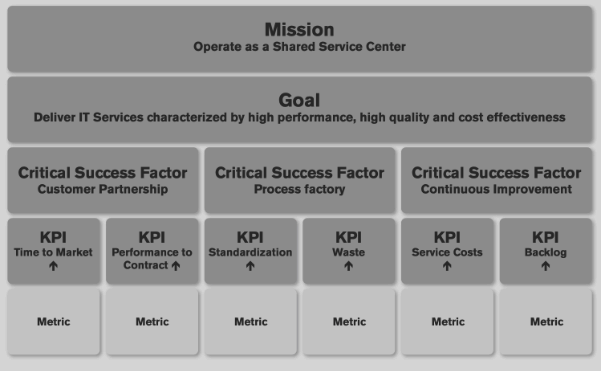
\includegraphics[width=0.9\textwidth]{images/vision.png}
    \caption{Organisational Vision}
    \label{fig:organizational_vision}
\end{figure}




